% !TEX root = multiplayer_reach_avoid_games.tex
\section{The Reach-Avoid Problem}
\subsection{The Multiplayer Reach-Avoid Game}
\label{sec:formulation}
Consider $\NA+\ND$ players partitioned into the set of $\NA$ attackers, $\pas = \{\pam{1}, \pam{2}, \ldots, \pam{\NA}\}$ and the set of $\ND$ defenders, $\pbs = \{\pbm{1}, \ldots, \pbm{\ND}\}$, whose states are confined in a bounded, open domain $\amb \subset \R^2$. The domain $\amb$ is partitioned into $\amb$ = $\free \cup \obs$, where $\free$ is a compact set representing the free space in which the players can move, while $\obs = \amb \setminus \free$ corresponds to obstacles in the domain. 

Let $\xam{i}, \xbm{j} \in \R^2$ denote the state of players $\pam{i}$ and $\pbm{j}$, respectively. Then given initial conditions $\xanm{i}\in \free,i=1,2,\ldots,\NA,\xbnm{i}\in \free,i=1,2,\ldots,\ND$, we assume the dynamics of the players to be defined by the following decoupled system for $t \geq 0$:

\bq\label{eq:dynamics}
\begin{aligned}
\dotxam{i}(t) &= \velai{i}\cam{i}(t), & \xam{i}(0) = \xanm{i}, i=1,2,\ldots,\NA \\
\dotxbm{i}(t) &= \velbi{i}\cbm{i}(t), & \xbm{i}(0) = \xbnm{i}, i=1,2,\ldots,\ND
\end{aligned}
\eq
where $\velai{i}, \velbi{i}$ denote maximum speeds for $\pam{i}$ and $\pbm{i}$ respectively, and $\cam{i},\cbm{i}$ denote controls of $\pam{i}$ and $\pbm{i}$ respectively. We assume that $\cam{i},\cbm{i}$ are drawn from the set $\A = \{\sigma \colon [0,\infty)\rightarrow \unitball \mid \sigma \text{ is measurable}\}$, where $\unitball$ denotes the closed unit disk in $\R^2$. We also constrain the players to remain within $\free$ for all time. Denote the joint state of all players by $\xj = (\xja, \xjb)$ where $\xja =(\xam{1},\ldots\xam{\NA})$ is the attacker joint state $\pas$, and $\xjb = (\xbm{1},\ldots,\xbm{\ND})$ is the defender joint state $\pbs$. 

The attacking team wins whenever $\m$ of the $\NA$ attackers reach some target set without being captured by the defenders; $\m$ is pre-specified with $0<M\le \NA$. The target set is denoted $\target\subset\free$ and is compact. The defending team wins if it can prevent the attacking team from winning by capturing or indefinitely delaying $\NA-\m+1$ attackers from reaching $\target$. An illustration of the game setup is shown in Fig. \ref{fig:mp_form}.

Let $\avoid_{ij} = \left\{\xj\in\amb^{\NA+\ND} \mid \|\xam{i}-\xbm{j}\|_2\le\Rc \right\}$ denote the capture set. $\pam{i}$ is captured by $\pbm{j}$ if $\pam{i}$'s position is within a distance $\Rc$ of $\pbm{j}$'s position. 

\begin{figure}
\centering
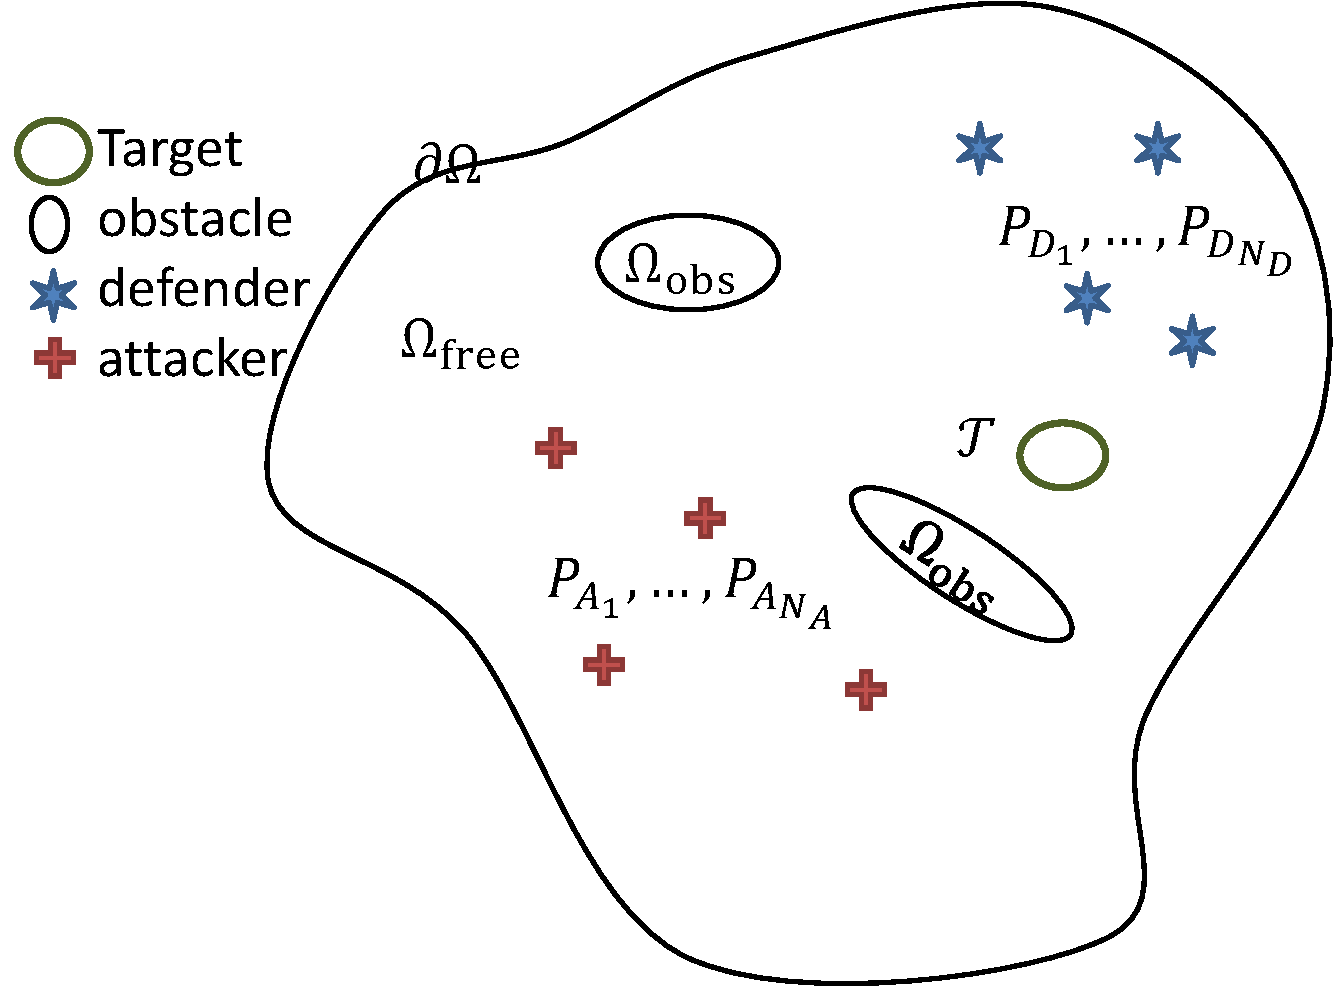
\includegraphics[width=0.35\textwidth]{fig/formulation}
\caption{The components of a multiplayer reach-avoid game.}
\label{fig:mp_form}
\end{figure}

In this paper, we address the following problems:
\begin{enumerate}
\item Given $\xjn$, $\target$, and some fixed integer $\m, 0<\m\le\NA$, can the attacking team win?
\item More generally, given $\xjn$ and $\target$, how many attackers can the defending team prevent from reaching the target?
\end{enumerate}

\subsection{The Two-Player Reach-Avoid Game}
\label{sec:2p_ra}
We will answer the above questions about the $\NA$ vs. $\ND$ reach-avoid game by using the solution to the two-player $1$ vs. $1$ game as a building block. In the two-player game, we denote the attacker $\pa$, the defender $\pb$, their states $\xa,\xb$, and their initial conditions $\xan,\xbn$. Their dynamics are
\bq
\begin{aligned}
\dotxa(t) &= \vela\ca(t), & \xa(0) = \xan,\\
\dotxb(t) &= \velb\cb(t), & \xb(0) = \xbn
\end{aligned}
\eq

The players' joint state becomes $\xj=(\xa,\xb)$, and their joint initial condition becomes $\xjn=(\xan,\xbn)$. The capture set becomes simply $\avoid = \left\{(\xa,\xb)\in\amb^2 \mid \|\xa-\xb\|_2\leq \Rc\right\}$. 

$\pa$ wins if it reaches the target $\target$ without being captured by $\pb$. $\pb$ wins if it can prevent $\pa$ from winning by capturing $\pa$ or indefinitely delaying $\pa$ from reaching $\target$. For the two-player reach-avoid game, we seek to answer the following:
\begin{enumerate}
\item Given $\xjn$ and $\target$, is the defender guaranteed to win? \label{p:tp1}
\item More generally, given $\xa$ and $\target$, what is the set of initial positions from which the defender is guaranteed to win? \label{p:tp2}
\end{enumerate}